%!TEX root = ../thesis.tex
%*******************************************************************************
%*********************************** First Chapter *****************************
%*******************************************************************************

\chapter{Introduction}

\ifpdf
    \graphicspath{{Chapter1/Figs/Raster/}{Chapter1/Figs/PDF/}{Chapter1/Figs/}}
\else
    \graphicspath{{Chapter1/Figs/Vector/}{Chapter1/Figs/}}
\fi

\section{Genetic variation}

\par{
Even before Gregor Mendel discovered the rules of genetic inheritance\cite{mendel}, the discovery that DNA was the molecule responsible for this\cite{Avery}, or its structure was known\cite{watsoncrick}, humans have wondered at the variation among each other and all organisms. These discoveries have since made way for a rapid expansion in our ability to measure genetic variation from capillary sequencing\cite{capillary} and single nucleotide polymophism (SNP) chips\cite{snpchip} to modern high throughput DNA sequencing\cite{bridgeamp} and long read sequencing\cite{HIFI}. We have sequenced thousands of individual humans and other organisms and explored the genetic variation of the human species \cite{1kgenomes}\cite{1kgenomes2}\cite{haplotypepanel}\cite{ukbiobank}\cite{hapmap}. We have used the genetic variation in population samples to impute population structure and evolutionary history\cite{NGSadmix}\cite{angsd}\cite{estimateadmixture}\cite{abbababa}\cite{shapeit4}\cite{beagle}. In this thesis, I explore computational methods for using genetic variation to resolve mixtures of haplotypes in single cell RNAseq, genome assembly, and scaffolding.
} 

\section{Introductiion}

\par{
In single cell RNA sequencing, the goal is not only to measure the transcriptome of many cells at a time, but also to compare the transcriptome of cells of different individuals or under different conditions such as disease state, pharmaceutical intervention, or a wide range of environmental differences. One problem with these comparisons is that there can be technical artifacts, or batch effects, between different experiments which bias the comparative results possibly even dwarfing the actual biological difference you are trying to measure. One solution to this problem is to pool the cells from different individuals into a single experiment. Additionally, single cell RNAseq has several sources of noise or errors (discussed in more detail in section \ref{section:scerrors}). One is when two or more cells are erroneously partitioned into the same compartment and the data for what is supposed to be one cell is actually two cells (doublets). And another source of noise is when RNA from previously lysed cells which are in solution with the cell suspension is sequenced along with the RNA from a patent cell and those reads are given the same cellular barcode (ambient RNA). In Chapter 2 of this thesis, I present a method for demultiplexing cells from mixtures of individuals into their individual of origin using the genetic variation measured in the single cell RNAseq reads without requiring prior knowledge of the genotypes. In addition, I show how---and provide methods for---how these mixtures improve doublet detection and ambient RNA estimation and removal.
} 

\begin{figure}[htbp!]
\begin{centering}

\caption{Outline of single cell clustering by genotype}\label{fig:souporcell}
\sidesubfloat[]{
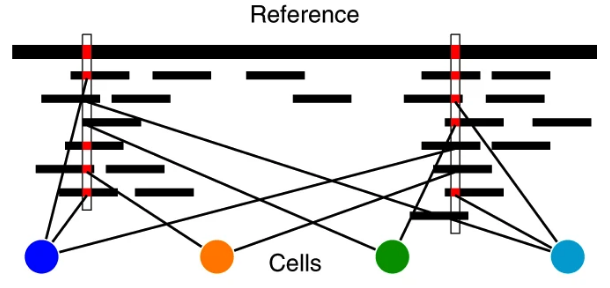
\includegraphics[width=0.3\textwidth, valign=c]{cellvariant.png} \label{fig:a}
}
\sidesubfloat[]{
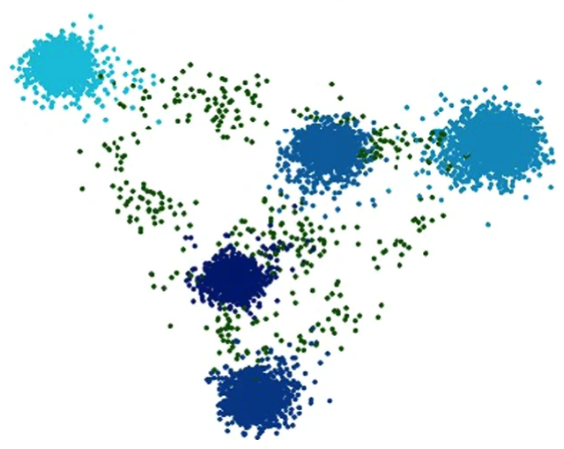
\includegraphics[width=0.3\textwidth, valign=c]{cellclust.png} \label{fig:b}
}
\sidesubfloat[]{
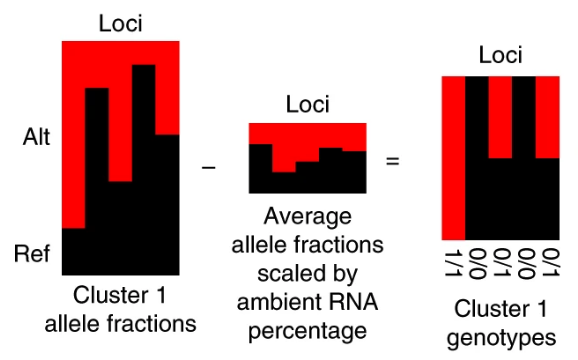
\includegraphics[width=0.3\textwidth, valign=c]{ambientrna.png} \label{fig:c}
}
\floatfoot{\small{\textbf{a)} We find the variants in the reads from each cell barcode, \textbf{b)} cluster cells by their allele content and identify doublets, and \textbf{c)} use the bias in allele fraction from expected values to estimate and remove ambient RNA.}}
\end{centering}
\end{figure}

\par{
In genome assembly, the goal is the use the overlapping read sequence similarity to infer that those reads came from the same locus in the genome and build contiguous sequences that represent (in part or whole) the organism's chromosomes. The inference that sequence similarity means these reads originated from the same genomic locus is complicated by repeats, heterozygosity, and sequencing errors. With inexact homology, one must disambiguate whether the differences arose from errors, paralogous repeat sequences, or from the alternate haplotype. If one cannot make this distinction and no reads span this region into more unique sequence, the contiguous sequence (contig) must be broken resulting in a fractious assembly. If the contig is not broken, one risks a chimeric misassembly of sequences that are distant to one another in the genome or on different chromosomes being assembled close to one another. In chapter 3 we discuss the first high quality assembly of a single mosquito. Prior to this, long read sequencing methods (discussed in section \ref{section:longreads}) DNA input requirement were too high to extract enough high molecular weight (HMW) DNA from many small organisms including mosquitos. This required pooling multiple individuals together in order to meet the DNA requirements for these sequencing technologies. Pooling individuals increases the number of haplotypes in the extracted DNA and makes distinguishing repeat from heterozygosity harder. Through recent advances in library preparation, the DNA requirements for long reads has been greatly reduced. By sequencing a single mosquito with long reads, we reduce the number of haplotypes from many down to two thus decreasing the potential ambiguities that arise from heterozygosity. We then compare this genome assembly to the current gold standard assembly of \textit{Anopheles gambiae} which was created using Sanger sequencing and bacterial artifical clones (discussed in section \ref{section:sanger}), a dramatically higher cost method of creating high quality genome assemblies. We show many improvement in our assembly over the previous gold standard as well as highlight several issues that remain with the current assembly state of the art.
} 



\par{
We continue to address the problem of heterozygosity in chapter 4 by showing several ways in which haplotype phasing consistency can be used as a signal for physical linkage. Given two or more proximate heterozygous loci, sequencing reads containing them should segregate into two groups according to which alleles they contain (assuming diploid). But how do we know that a site is heterozygous. Initially we do not. We can find sequence which has inexact homology each being read roughly half of the times general homozygous sequences occur. These could be due to heterozygosity or paralogous sequences both with low occurrence by chance due to random sampling. In both cases, reads containing multiple of these alleles should segregate into two (assuming copy number of the repeat is two) groups. But when comparing a true heterozygous site with inexact homologous sequence caused by paralogous sequence, the reads with both alleles of the heterozygous site will contain one of the presumed alleles caused by the repeat sequence. We can use this property in both assembly and scaffolding to avoid misassemblies, create phased assemblies, and scaffold contigs in a phasing aware fashion. In chapter 4, we outline how we go about finding candidate heterozygous sequences in a \textit{de novo} way, the phasing consistency criteria, how we build a phased assembly graph, and can separate reads by their haplotypes prior to haploid assembly. We also show how to use this same property for scaffolding using long range genetic information from linked reads and HiC (discussing in sections \ref{section:linkedreads} and \ref{section:hic}). In case the assembly we wish to scaffold was not built by our phased assembly method, we also provide an algorithm for haplotype phasing the \textit{de novo} candidate heterozygous sites within each contig which is a requirement for phasing aware scaffolding. This tool has the added benefit of being robust to being given non heterozygous sequences as input and can use the phasing inconsistency to correct the genotypes. We demonstrate these techniques on data from the butterfly \textit{Vanessa atalanta}.
} 

\begin{figure}[htbp!]
\begin{centering}

\caption{Phasing consistency as a \textit{de novo} signal for physical linkage}\label{fig:phasstools}
\sidesubfloat[]{
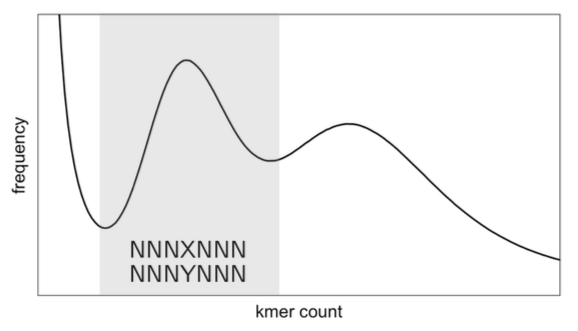
\includegraphics[width=0.3\textwidth, valign=c]{spectrum.png} \label{fig:a}
}
\sidesubfloat[]{
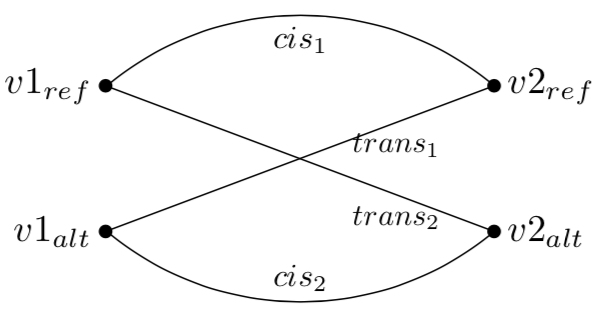
\includegraphics[width=0.3\textwidth, valign=c]{consistency2.png} \label{fig:b}
}
\sidesubfloat[]{
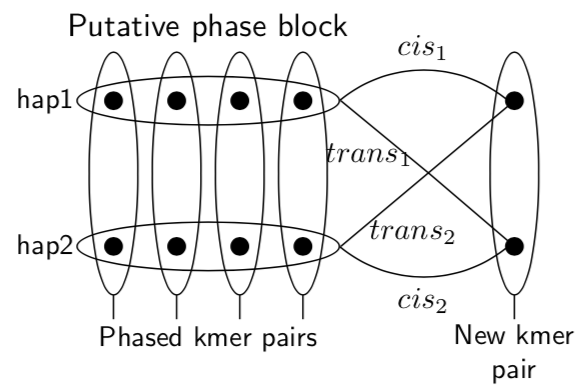
\includegraphics[width=0.3\textwidth, valign=c]{consistency3.png} \label{fig:c}
}
\floatfoot{\small{\textbf{a)} We use the kmer count spectra to determine candidate heterozygous kmer pairs which we can then \textbf{b)} assess for phasing consistency based on the alleles on reads that contain one of each, and \textbf{c)} build a phased assembly graph.}}
\end{centering}
\end{figure}

\par{
The remainder of this chapter contains the background and context for this work. I first cover the history of single cell sequencing and analysis. I then outline the biases and errors that occur in single cell sequencing and the various solutions and their downsides which motivates chapter 2. I then go over the history of DNA sequencing methods as well as assembly and scaffolding algorithms. I discuss the inherent ambiguities that can occur and the errors that can arise and their causes which motivates chapters 3 and 4.
}

\section{Single Cell RNAseq}

\par{
The etymology of the word cell comes from the latin \textit{cella} meaning storeroom or chamber. These entities separate the physical space between what is life and nonlife, first discovered by Robert Hooke in 1665\cite{Hooke}. This partitioning the cell provides is necessary for life due to the second law of thermodynamics and the nature of life. In Erwin Schrodinger's classic lecture series and book titled ``What is Life''\cite{whatislife}, he noted that while closed physical systems will always tend toward increased entropy (stated by the 2nd law of thermodynamics\cite{thermodynamics1}\cite{thermodynamics2}\cite{maxwell}), life must maintain (on average) a neutral or negative entropy in the portion of the system in which it resides\cite{informationtheorylife}\cite{astrobiology}\cite{extremalities}. In order to do so, this requires the expenditure of energy. Biological evolution found an economical way of solving this problem with the bilipid membrane with various embedded molecules giving it the property of semipermeability---allowing some molecules in and not out or vice versa in a dynamic fashion. These cells proved, over time, to be so successful as to become the primary unit and building block of biological life on this planet. Incidentally, Erwin Schrodinger, as the father of quantum mechanics, along with Josiah Gibbs, as the father of statistical mechanics, will appear again later in this thesis as some of the algorithms described take ideas inspired by these fields for search strategies in optimization problems.
} 

\par{
When studying the state of a cell and its current function, we could try to measure many different properties such as the proteome, transcriptome, genome, chromatin accessability, environmental conditions (such as hormone content, PH, etc), cell surface proteins. But we are somewhat limited by the tools available, and when addressing function, we first turn to the central dogma of molecular biology\cite{centraldogma} that states that information in general passes from DNA to RNA and then to proteins. If we could easily inspect the protein content of many cells in a high throughput fashion, that would be desirable, but protein detection and sequencing methods often only limited to one or a few proteins at a time and/or are not high throughput\cite{immunohistochemistry}\cite{multiIHC}\cite{westernblot}\cite{western2}\cite{multimassspec}\cite{ionbeam}\cite{cellIHC}\cite{proteinsequencing}. But we do have a very high throughput detector for DNA and can convert RNA into complementary DNA (cDNA).
}

\subsection{Bulk RNAseq}
\par{
Scientists have been sequencing cDNA libraries of RNA isolated from many cells mixed together since the advent of next generation DNA sequencing technologies (discussed in section \ref{section:nextgen}) became available\cite{RNAseq1}\cite{RNAseq2}. Because these use extractions from pools of cells, they are denoted as `bulk' RNAseq. These experiments have provided many discoveries, but are limited in their usefulness because they represent the average transcriptome across a population of potentially diverse cells. This blurs the data and makes inference on minority cell types difficult if not impossible. The amount of RNA in a single cell is roughly 10-30pg\cite{howmuchrna} which until recently was not enough to create a complex cDNA library from even with amplification. Some researchers have isolated specific cell types using Fluorescence Activated Cell Sorting (FACS)\cite{FACspatent}\cite{FACs} prior to RNAseq to some success\cite{FACszebra}, but due to FACS cell stress and it only accessing one cell type at a time it is of limited usefulness.
}

\subsection{Single cell RNA sequencing}

\par{
In the past decade, technical advances in methods for the preparation of samples containing minuscule amounts of nucleic acids have made it possible to study the transcriptome of single cells\cite{first_singlecell} and have changed the way biologists can access the functional state of individual cells within a complex and diverse population of cells in tissues across different states of organisms shedding light on the cellular response to diseases, drugs, development, and more.
} 
\par{
There are many types of RNA in the cell including messenger RNA (mRNA), transfer RNA (tRNA), ribosomal RNA (rRNA), micro RNA, and small nucleolar RNA. mRNA makes up only 3-7\% of the cell's total RNA by mass\cite{rnacontent}, but it is what is translated by ribosomes into proteins, which conduct a large amount of the function of the cell. Single cell RNA sequencing targeting other types of RNA have also been developed for alternative types of RNA for specific purposes\cite{nonmRNASC}, but in this thesis when referring to single cell RNAseq (scRNAseq) we are talking about a system that enriches for mRNA by using the 3' polyadenylation most mRNAs have (with some exceptions\cite{nonpoly}).
}

\subsection{Technologies}

\par{
mRNA from a single cell was first isolated and amplified to measurable levels with polymerase change reaction (PCR)\cite{PCR}\cite{PCRPatent} in the early 1990s\cite{earliersinglecell} before the sequencing revolution. Without a high throughput detector, and due to the exponential nature of PCR causing abundant mRNA to dominate the sample, very few genes are detected. This increased with linear amplification achieved by multiple cycles of transcription of antisense RNA from the initial cDNA using T7 RNA polymerase\cite{T7amp} and the advent of oligonucleotide microarrays\cite{snpchip} allowing for RNA microarray studies detecting over a thousand genes\cite{microarrayRNA}\cite{microarraySC2}. However, the number of genes measured were still a fraction of the total genes expressed. The first sequencing of single cell cDNA sequencing increased the number of genes detected by 75\%\cite{first_singlecell} and provided a hypothesis free measurement of the transcriptome a single cell. Since then, single cell RNAseq has grown greatly in the number of cells processed per experiment, the number of genes detected per cell, and its uptake by the scientific community\cite{singlecellgrowth}.
}

\par{
Current scRNAseq protocols convert RNA to cDNA using a reverse transcriptase primed off of the poly-A tail of the mRNA. At the same time, a cellular barcode as well as template switching oligo (for subsequent PCR) are added. Often, a unique molecular identifier (UMI) is also added. This is used to know which cDNA molecules were amplified from the same RNA source molecule to avoid counting PCR duplicates multiple times\cite{UMI1}\cite{UMI2}. This reduces the PCR biases versus a simple read counting strategy. 
} 

\par{
To deliver a barcode oligo to all of the reads originating from one cell and different barcodes to different cells, physical separation of one form or another is generally used. The separation could be in different tubes, plate wells, nanowells\cite{seqwell}\cite{scalablemicro}\cite{combilabel}, or more recently with microfluidic systems creating a reverse emulsion droplets\cite{dropseq}\cite{Klein2015}\cite{10xsinglecell}. These methods vary in several parameters including the scalability of number of cells per experiment, the capture rate of mRNA, and the technical variation between experiments among others\cite{powersingle}\cite{singlecompare}\cite{singlecompare2}. Which method is best to use ultimately depends on the biological question. For experiments where sampling the whole population of cells is important, droplet and nanowell methods are better whereas if capture rate and amount of data per cell, plate based systems would be better. 
}

\subsubsection{10x genomics}

\par{
In this thesis, all of the single cell data used was generated using the 10x genomics chromium platform, a reverse emulsion droplet based system. Figure \ref{figure:10xsinglecell} outlines how this system works. It uses a microfluidic system to deliver gel beads, reagents, and cells into reverse emulsion droplets where the reverse transcription occurs. The gel bead contains oligos with the cell barcode, a UMI, and primers for the PCR and Illumina sequencing\cite{10xsinglecell}\footnote{I was fortunate to have worked at 10x Genomics between 2014 and 2017. While I did not work much directly on the single cell technology (I primarily worked on the company's first product, linked reads), I gained much insight into the data by being present for its creation.}.
}
\begin{figure}[htbp!]
\caption{10x Genomics single cell RNAseq}
\label{figure:10xsinglecell}
\begin{centering}
\sidesubfloat[]{
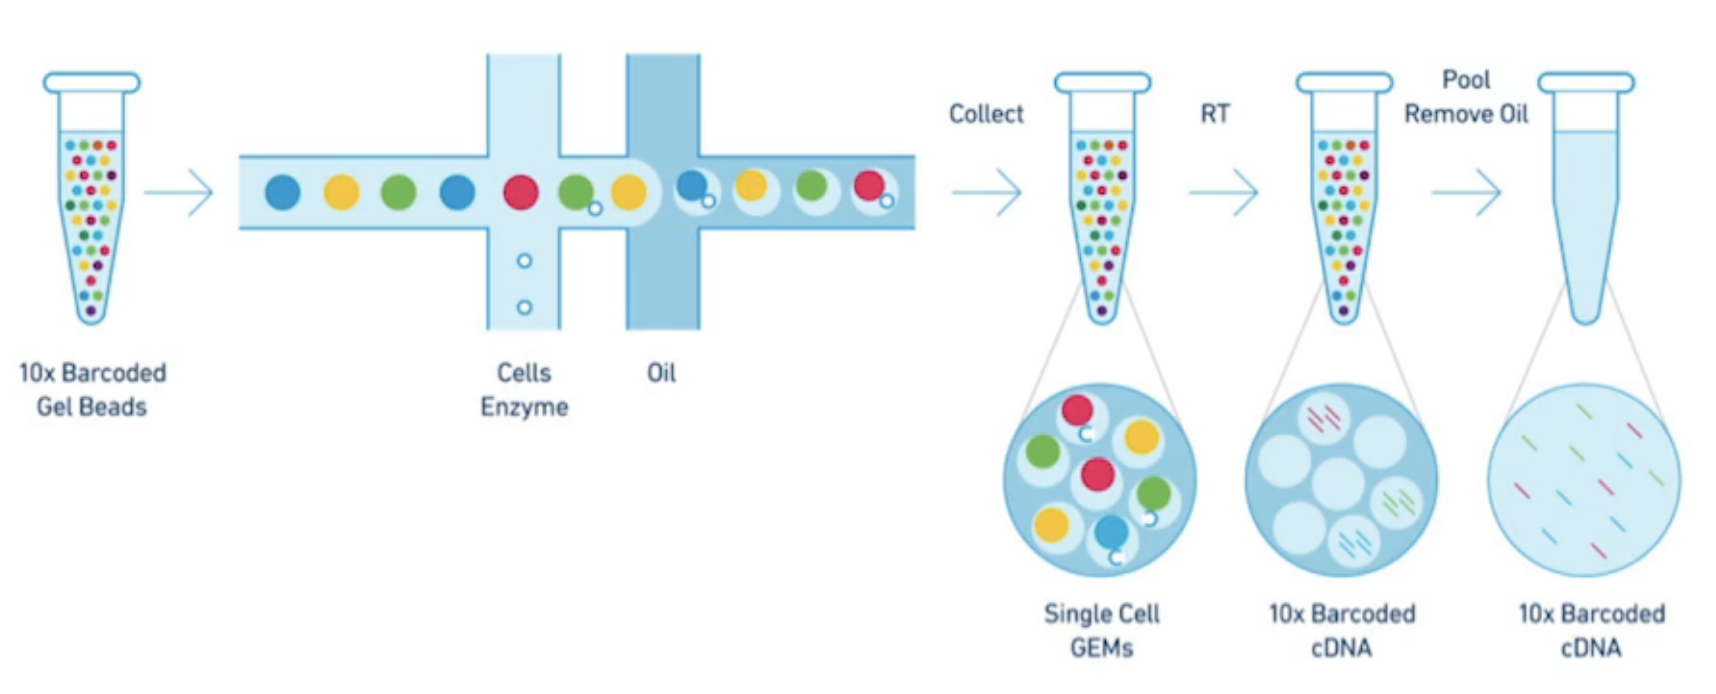
\includegraphics[width=0.85\textwidth]{singlecelloverview2.png}} \\
\sidesubfloat[]{
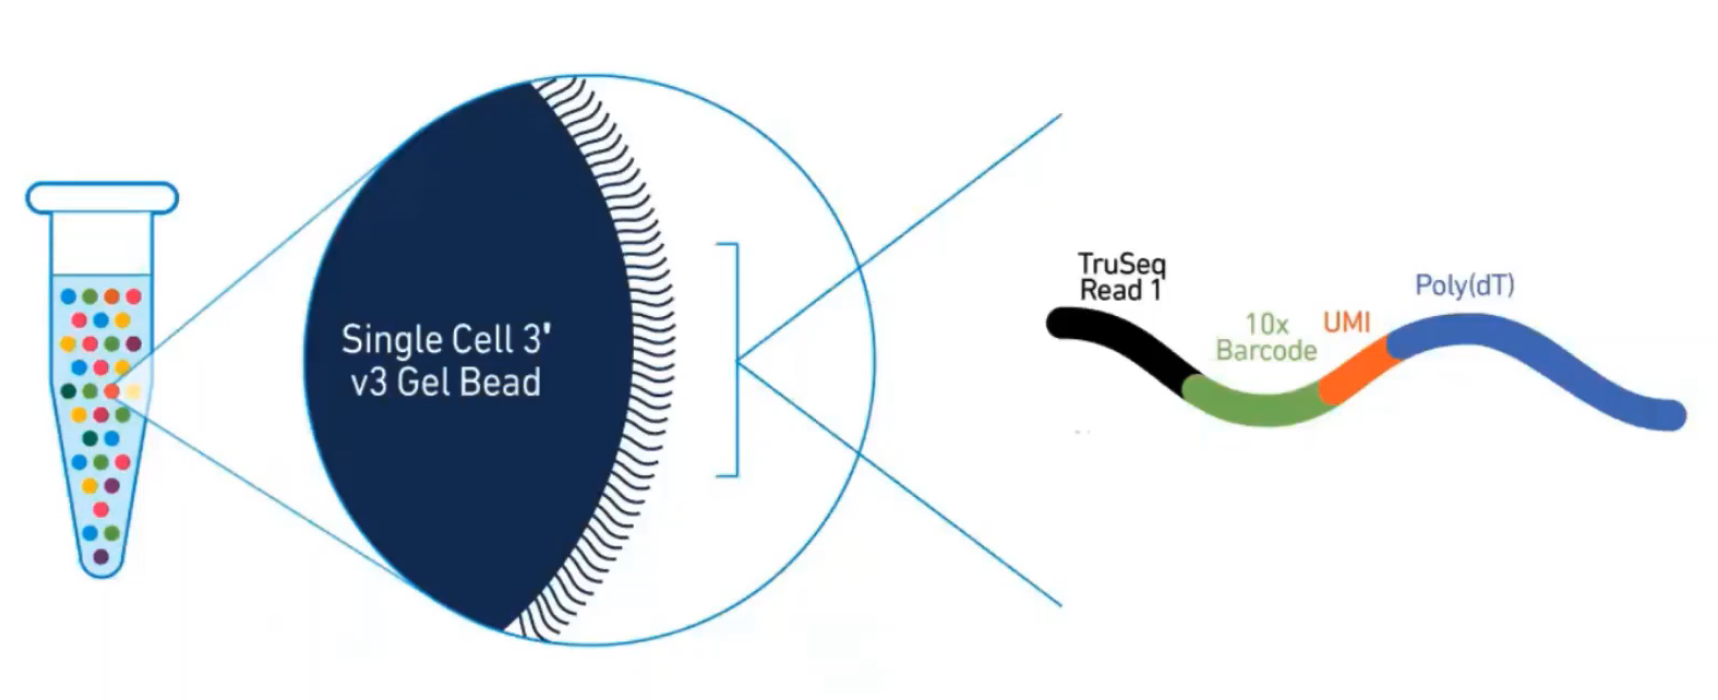
\includegraphics[width=0.85\textwidth]{singlecell2.png}
}
\floatfoot{\small{Diagram outlining 10x Genomics single cell sequencing technology (credit: 10x genomics website).}}
\end{centering}
\end{figure}

\subsection{Analysis of scRNAseq data}

\par{
This construct is then sequenced on a next-generation Illumina sequencer \cite{bridgeamp}\cite{illuminareview} (discussed in detail in section \ref{section:nextgen}) giving paired-end reads with one read containing the cell barcode and UMI and the other read containing the cDNA of the mRNA transcript. Other sequencing platforms have been used, notably long read sequencing platforms to get the whole transcript read to investigate alternative isoforms, but will not be discussed further here\cite{tilgner}\cite{isoformseq}\cite{longreadsinglecell}. The most common software package used to go from the sequence files to cell gene counts matrix and initial cell type clustering is cellranger\cite{cellranger} and while alternatives exist\cite{dropseqsoft}, they do largely the same steps. 
}

\subsubsection{Genome alignment}

\par{
First, the template switch oligo and polyadenylation are trimmed from the 5' and 3' ends of read two respectively. Then the read two is mapped to the given reference genome using the STAR splicing aware RNA aligner\cite{STAR}. Other aligners exist for this purpose such as HISAT2 \cite{hisat} and TopHat2 \cite{tophat2}. Also there are psuedo-aligners (Kallisto\cite{kallisto} and Salmon\cite{salmon}) which are much faster and robust to sequencing errors but do not provide spicing information\cite{alignfree}. The reads are then marked as exonic or intronic using the given transcript annotation gene transfer format (GTF) file and confident or not based on if the read overlaps an exon for >50\% of its length and if the mapping quality (mapq) is 255 which indicates that the read aligned uniquely to one location. Confident exonic reads are carried forward to the UMI counting step\cite{singlecelloverview}.
}

\subsubsection{Barcode correction}
\par{
Before counting UMIs, cellranger attempts to do barcode correction on the cell barcodes. 10x Genomics uses a designed barcode set of either 737 thousand or 3 million barcodes each with a hamming distance\cite{hamming} of at least two to any other barcode in the set. The barcodes that make up this designed set are the barcodes we expect to see and this set is termed the whitelist. In order to error correct barcodes, first the frequency of each barcode in the whitelist is counted. Then for every barcode that is not in the whitelist, each sequence that is one hamming distance from this sequence and is on the barcode is found. A posterior probability is computed with the priors set by the frequency of that whitelist barcode and the base quality of the changed base used to determine likelihood of that error. For a barcode correction to then take place, the posterior probability of that whitelist barcode must be over 97.5\%\cite{barcodecorrection}.
}

\subsubsection{UMI counting}

\par{
PCR duplicates are then removed using the cell barcode, UMI, and gene. If any reads have the same three, all are discarded except one. The remaining reads will be counted to create the cell barcode by gene count matrix. Note that not each cell barcode contains a cell. Due to ambient RNA in solution from cells lysed before reverse emulsion partitioning, droplets without a patent cell will have some reads. We next need to determine which cell barcodes have cells and which do not.
}



\subsubsection{Cell-barcode detection}
\par{
Initially, cell containing GEMs were called using the second derivative of the log-log UMI counts by barcodes plot (see figure \ref{figure:knee}). More recently, a method using the RNA content of the confidently empty droplets called EmptyDrops\cite{emptydrops} was developed to compare that RNA content (which is generally an average of the RNA content of all cells assuming each cell type lyses with equal probability) with the RNA content of the cells to determine an appropriate cutoff where the difference from the average decreases rapidly. This particularly helps in situations where the cell population contains some cells with a large amount of transcription and another cell type with many fewer transcripts. Both of these cell types will likely still have a very different transcriptional profile than the empty droplets. This algorithm has now been implemented in cellranger. The raw cell barcode by genes UMI counts matrix is then filtered to retain only cell containing cell barcodes.
}
\begin{figure}[htbp!]
\caption{Cell barcode detection knee plot old vs new algorithm}
\label{figure:knee}
\begin{centering}
\sidesubfloat[]{
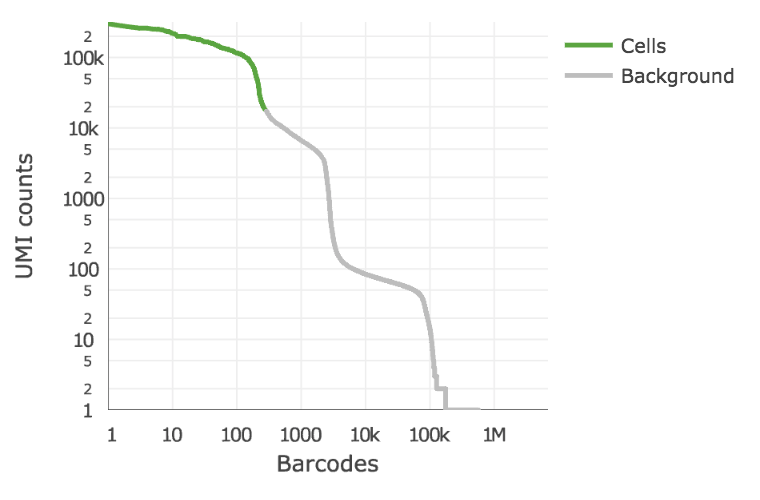
\includegraphics[width=0.45\textwidth]{knee1.png}} 
\sidesubfloat[]{
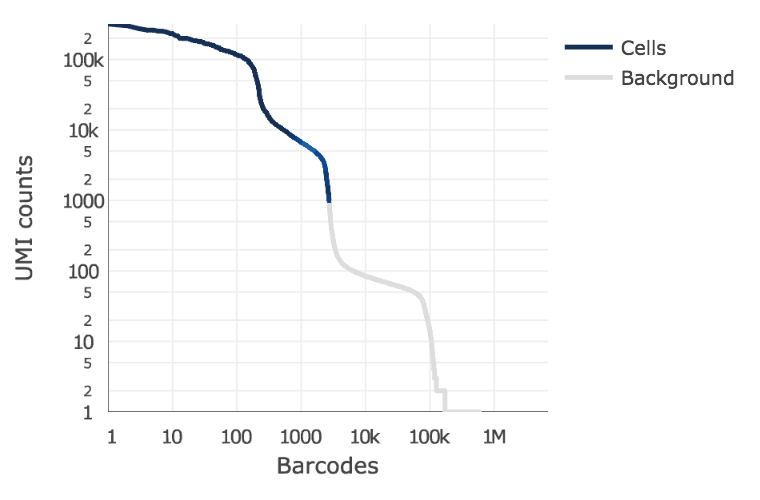
\includegraphics[width=0.45\textwidth]{knee2.png}
}
\floatfoot{\small{Log-log barcode by UMI count knee plots showing which barcodes were determined to contain cells under the \textbf{a)} old method using 2nd derivative and the \textbf{b)} new EmptyDrops method (credit: 10x genomics website).}}
\end{centering}
\end{figure}

\subsubsection{Quality control}

\par{
Many of the following steps are done in software packages downstream from cellranger which aim to implement many types of analyses for scRNAseq data. The most popular of these software packages is seurat\cite{seurat1}\cite{seurat2} and while alternatives such as Monocle\cite{monocle}, a comparison is out of the scope of this thesis.
} 

\par{ In the process of cell dissociation, liquid handling, and partitioning, some cells may be damaged. For this reason, many researchers use different criteria to remove these poor quality cells. Some also use different criteria for different cell types and so a less stringent global filter may be applied prior to cell type detection and further filtering. These criteria include number of genes per cell, \% mapped reads, \% reads that map to spike in controls, \% mitochondrial reads, and \% of reads that are PCR duplicates. While these are reasonable markers for dead or dying cells\cite{osorio}\cite{ilicic}, it is my personal opinion that this type of quality control should be limited and standardized as much as possible to prevent unintentional bias in the results affecting how these thresholds are chosen. 
}

\subsubsection{Normalization}\label{section:normalize}

\par{
As previously discussed, individual cells have extremely small amounts of mRNA and require methods to amplify this material in order to be made into a cDNA library and sequenced. These methods, along with the innate difficulties of measuring such a small amount of starting material inevitably result in some technical artifacts. Genes that are expressed to a lesser degree than other genes may show zero counts or lower than true counts in the experiment for several reasons\cite{technoise}. Capture rate of mRNA in the reverse transcription step will never have complete yield and may vary from cell to cell and gene to gene. Additionally, genes that are expressed might be made into cDNA and amplified, but not sampled in the sequencing step as transcripts that begin with a higher copy number get amplified more in the exponential PCR step. Differences in cell size, and thus mRNA content, may result in sampling of genes in one cell type not sampled in other cell types even if both express them. To address this, many normalization methods have been developed\cite{normalize1}\cite{normalize2} to address these problems. Spike in controls can be used to improve this normalization\cite{marioni1} but takes up valuable sequencing. Another solution is imputation\cite{imputesc}, but this can introduce unwanted false positives\cite{fpimpute}. In the comparison papers, differential expression has been shown to be the downstream application most sensitive to these methods\cite{normalsc}, with scran\cite{scran} performing the best of those tested.
}

\subsubsection{Visualization}

\par{
In order to visualize this high dimensional data, we must project it into two or three dimensions in a way that preserves the biologically interesting structure at multiple scales. First, a principle component analysis (PCA) of the filtered cell by genes counts is done to find the most meaningful features and reduce the dimensionality from cells x genes to cells by $M$ where $M$ is a user settable value\cite{pcaimpl}. For most experiments, the complexity of the transcriptional profile cannot be easily gleaned by looking at the first two-three principle components visually, so the next step is to use non-linear dimensionality reduction techniques to bring the data into a visually informative two or three dimensional space. The two most popular methods for this are the t-Stochastic Neighbor embedding (t-SNE)\cite{tsne1}\cite{tsne2}\cite{hinton} and the Uniform Manifold Approximation and Projection (UMAP)\cite{umap1}. Both of these methods aim to preserve pairwise distances in the final projections, but are parametric and non-deterministic (without a fixed psuedorandom number generator seed). There is an inherent trade-off between how well distances should be preserved at different scales which the parameters can help guide. However, due to the randomness and parametric nature of these algorithms, it can lead some researchers to use them to bias the results toward the expected outcome of their hypothesis. Nonetheless, these are powerful techniques to understand high dimensional data such as single cell RNAseq. Recently, UMAP has grown in popularity over t-SNE because it has been shown to better preserve pairwise distance due to the improved initialization strategy employed in the primary implementation and is more computationally efficient than t-SNE\cite{umap2}\cite{umap3}. These projections are often fed into downstream analysis such as clustering and lineage reconstruction. It is not clear that clustering in this space is better than clustering on the raw data, PCA, random projection\cite{randomproject}, or other dimensionality reduction space, but they are likely to look more visually correct in the UMAP or t-SNE space when both the clustering and visualization is in the same projection. An analysis of this observation is out of the scope of this thesis.
}


\subsubsection{Cell type clustering and annotation}

\par{
It is useful to group similar cells together for the purposes of cell type annotation and cell state detection. Because individual cells may not have enough UMIs sequenced, these analyses may not be possible on an individual cell basis whereas grouping similar cells together will pool enough data to conclusively do so. Clustering is typically done on the dimensionality reduced data (either PCA or UMAP/t-SNE) and many methods have been used including K-means, hierarchical clustering, graph based methods and meta-heuristics have been applied including consensus clustering, cluster trees among others\cite{scclustreview}\cite{subpop}\cite{sc3}\cite{clustree}. These methods are reviewed in \cite{scclustreview} and otherwise a comparison of these methods is out of the scope of this thesis.
} 

\par{
Once cells have been clustered into similar groups, we can try to understand what each of these groups of cells represent. Marker genes have been studied for many decades to identify and differentiate different cell types. One can visually display the expression values of these marker genes versus the cell clusters to find the cell types of interest. Increasingly more popular are automatic methods which use annotated cell atlases to match cell types. These include scMatch\cite{scMatch}, cellHarmony\cite{cellHarmony}, Garnet\cite{Garnet}, scPred\cite{scPred} with some using prior knowledge of marker genes and some not. A comparison of these methods found that they work fairly similarly with scPred performing the best overall. Interestingly, they find that prior knowledge of marker genes does not improve performance. Other methods allow you to project cells from one dataset onto another\cite{scmap}. For systems which have robust prior annotated datasets, these are powerful and accurate tools for automatic annotation.
}



\subsection{Downstream analysis}
\par{
Many further analyses on single cell experiments are possible and a comprehensive review of these is out of the scope of this thesis. Pseudotime analysis can order cells along some cell state change such as differentiation or cell cycle\cite{pseudotime}\cite{scHOT}. Gene regulatory networks may be inferred using the correlation of genes indicating they may be under similar regulatory control\cite{scenic}. Somatic mutations in the mitochondrial genes can be used to discover cell lineages\cite{lineage}. And many more analyses are possible especially if the experimental design is non-standard such as multi-Omic single cell sequencing or CRSPR-Cas9 screening\cite{perturb} etcetera is added to the mix.
}

\subsection{scRNAseq error modes}\label{section:scerrors}

\subsubsection{Batch effects}

\par{
Due to the manner in which scRNAseq data is created, it naturally has certain noise and error characteristics. In section \ref{section:normalize}, we discussed intra-dataset technical artifacts. Naturally, inter-dataset technical artifacts are larger in magnitude and more diverse. If any of the laboratory protocols were changed, or the experiment was done by a different person, on a different day, at a different temperature, etcetera, it may introduce inter-dataset differences which may be even larger than the biological differences we wish to measure. There are a multitude of computational methods to correct these batch effects such as scanorama\cite{scanorama}, mnnCorrect\cite{batch1}, BBKNN\cite{BBKNN}, Harmony\cite{harmony}, Seurat\cite{seurat3}, and LIGER\cite{LIGER}. Each of these either finds matching cell populations or overall data correlations to then create a projection to bring the datasets into a common space. A comparison study tested 14 of these methods and evaluate the adjusted rand index of cell type clustering, average silhouette width of cell type clustering, and two other metrics and found that Seurat, LIGER, and Harmony performed best. While these are powerful tools for correcting these technical variations, it is possible that in trying to correct for variation due to batch effects that some biological differences will also be erased or biased.
}

\subsubsection{Doublets}

\par{
In 10x genomics, the loading of droplets with cells is a random process which follows a poisson sampling distribution. The experiments are designed with a cell suspension concentration to produce a poisson distribution with a mean much less than one. This results in an experiment in which most droplets sample zero cells and some sample one cell. But in order to collect enough cells, that mean still must not be vanishing small. So some droplets will sample more than one cell. These cell barcodes which are associated with more than one cell are generally called doublets though multiplets might be more appropriate as some may have more than two cells. Another way that these arise is if the tissue dissociation of cells was not complete or if there is any cell adhesion causing cells to travel together in suspension. Again, a number of computational tools have been developed to find and remove these doublet cell barcodes from further analysis. These include doubletCells\cite{doubletCells}, DoubletFinder\cite{doubletfinder}, Scrublet\cite{scrublet}, DoubletDecon\cite{doubletdecon}, scDblFinder\cite{scDblFinder}, and Solo\cite{solo} among others. Many of these use simulated doublet by combining in silico the UMI counts of putative singleton cells to identify what the transcriptional profile of a doublet would look like. Validating these methods is somewhat problematic as in real datasets, the doublets are not known, and simulated doublets may not exactly match what data would look like from true doublets. In a recent benchmark of these methods, many of these performed similarly with scDblFinder scoring the highest overall\cite{doubletbench}. Once again, these are powerful methods, but do not work flawlessly and in particular may remove cells in an intermediate state transition between two more distinct cell types in the sample so may remove cells of potential interest.
}


\subsubsection{Ambient RNA}

\par{
Another aspect of scRNAseq data that biases our view of the transcriptional landscape is ambient RNA. Before the cells are partitioned, some cells may have lysed, or there may be other cell free RNA in solution. This RNA will be delivered to all droplets including droplets that contain a cell and that RNA will be sequenced with the same cell barcode as the reads that truly came from the cell. This is alternately called ambient RNA or the `soup'. Ambient RNA can be analyzed by looking at the reads from non-cell barcodes and is generally an average of all of the RNA in the experiment, but this is not always true such as when some cell types are more prone to lysing than others or samples such as necrotic tumor. The amount of ambient RNA in the system is generally small, but may be increased in some samples such as tissues which requires harsh detergent agents to be used to dissociate the cells into a cell suspension. SoupX was developed in order to estimate the amount of ambient RNA and remove it\cite{soupx}, but requires prior knowledge of gene expression in different cell types as it uses measurement of genes known to not be expressed in certain cell types to measure the ambient RNA. 
}

\subsubsection{Mixtures}

\par{
One experimental design that promises to solve all three of these error modes in scRNAseq are mixture experiments. If cells from multiple samples are mixed together, you limit the number of technical artifacts between them to differences in how the cells were treated prior to being mixed. If you can distinguish which cells came from which samples, you can use that same signal to determine which cell barcodes represent cross-sample doublets. And depending on the sample features, this may also aid in measuring ambient RNA. Several experimental methods have been developed to tag cells by sample prior to mixing. Cell hashing uses oligonucleotide tagged antibodies attached to cell surface proteins as a sample signal\cite{cellhashing}\cite{nucleimulti}. MULTI-seq uses lipid and cholesterol modified oligonucleotides which incorporate into any lipid membrane to generate a sample read-out\cite{multiseq}. CellTag uses heritable genetic material as a sample index for tracking cells through passages after mixing to better study sample interactions\cite{celltag}. These are powerful methods for reducing batch effects, detecting doublets, and reducing costs through both multiplexing and giving more scope for overloading the number of cells per experiment. As the number of cells per experiment is increased, the number of doublets grows as well. If one has a robust method of identifying and removing doublets, one can load more cells and recover more singletons even after removing the doublets. However, there is a limit to this. 10x genomics reports that the number of doublets is roughly 1\% per thousand cells recovered. This is of course an oversimplification. If the cell suspension is fully dissociated, the cell loading is a poisson process. In the range of two to ten thousand cells, this generates roughly 1\% doublets per thousand cells. Outside of this range, this rule falls apart. One can, however, fit a poisson to a number of different experiments with differing number of cells for a better model. Over some number, the marginal increase in singletons recovered as more cells are added decreases and at some point actually diminishes. This is also worsened by the fact that the doublets and multiplets take up valuable sequencing only to be discarded. Additionally, doublet detection methods are not perfect and the remaining doublets will bias your experimental results. 
} 

\par{
But these methods require additional experimental work and are not always possible. Some mixture samples are naturally occurring such as at the maternal/fetal boundary, transplant patient tissue, or complex multiple infections. If the mixed samples have distinct genotypes, one can use the genetic variation between samples to demultiplex them. Demuxlet was first developed for this purpose, but requires prior knowledge of the genotypes of each sample and its rigid model based system can make errors especially as the amount of ambient RNA in the system increases\cite{muxseq}\cite{demuxlet}. In chapter 2, I present souporcell, a method for clustering cells by genotype without prior knowledge of each sample, cross sample doublet detection, and ambient RNA measurement. We compare our system against Demuxlet and two other methods, scSplit and vireo\cite{scsplit}\cite{vireo}, across a wide range of challenging datasets. Since then, freemuxlet was developed as another such method, but is not compared to as it came out later and is unpublished outside of a thesis\cite{freemuxlet}.
}

\section{Genome assembly and scaffolding}
\par{
Since Mendel's discovery of the laws of heritability\cite{mendel}, it has been a goal to link the micro to the macro to explain evolution in a quantitative fashion\cite{evolutionmicro}. The discovery that DNA encoded the hereditary information of organisms\cite{Avery} and subsequent discovery of its chemical structure\cite{watsoncrick} made clear the nature of information storage in a linear polymer and mechanism for stable replication. Even before the discovery of mRNA\cite{mRNA1}\cite{mRNA2}, Francis Crick hypothesized that nucleic acids direct the synthesis of proteins\cite{proteinsynthesis} and later elucidated what is now known as the central dogma of molecular biology\cite{centraldogma1}. In brief, this states that the information flow of an organism is through the DNA being transcribed into RNA and the RNA translated into proteins which perform most of the functions of the cell. With the information source being the DNA, this made clear the importance of reading the sequence. And for several decades, our ability to read DNA sequence has dramatically increased in both amount and accuracy.
}

\subsection{DNA sequencing}

\par{
The history of DNA sequencing is generally thought of as having three waves---Sanger sequencing, next-gen sequencing, and third generation sequencing. Sanger sequencing is highly accurate and relatively long reads at 500bp to 1kb but is not very scalable. Next-gen sequencing produces high accuracy short reads (initially 35bp, but now can be up to 250bp) and is massively scalable. At the same time, many other sequencing technologies came along without much success. In the third wave, the ability to sequence long reads of single molecules without amplification has transformed genome assembly. Pacbio and oxford nanopore developed single molecule long read sequencers that produced low accuracy (85 and \~90\% respectively) long reads limited mostly by the input DNA length and stability. More recently, Pacbio utilizes circular consensus sequencing to produce reads in the 5-25kb with high accuracy. Other technologies in the third way employ different methodologies for getting long range genetic information but are sequenced with the high throughput and low cost next-gen sequencers.
}

\subsubsection{Sanger sequencing}\label{section:sanger}

\par{
The ability to sequence proteins and certain RNA molecules came before the ability to sequence DNA due to proteins being made of more diverse monomers and RNA not being complicated by a complementary strand\cite{aminoacidsequence}\cite{sequenceofsequencers}. In 1965, Robert Holly and Frederick Sanger developed two related methods for sequencing RNA\cite{Holly1}\cite{Sanger1}. These were labor intensive and Sanger's method employed dangerous radioactive material. This method was then extended to DNA in 1973 and used to sequence 50 bases of the phage f1\cite{Sanger2}. Eventually, the use of polyacrylamide gel electrophoresis, chain termination chemistry with dideoxynucleotides, the use of flourescence instead of radiolabeling, and automation brought us to what is know known as Sanger sequencing\cite{Sanger3}. This technology was automated and became the most popular method of sequencing for many years\cite{Hunkapiller1991}. These sequences are highly accurate as each base signal is the result of the termination of a many molecules and have read lengths from 500bp to 1000bp which is limited by reaction efficiency requiring a fraction of chain terminations at every base of the sequence. This method requires clonal DNA and thus laboratory methods were developed for creating libraries for sequencing. BACs and YACs \cite{BACsYACs} were developed and each end could be sequenced creating a mate pair read spanning hundred of kilobases giving long genetic distance linking information.
}

\subsubsection{Short reads}\label{section:nextgen}

\par{
In the poorly named ``next-gen'' phase of DNA sequencing, there were many technologies created, but ultimately one became the dominant one and discussing each in detail is out of the scope of this thesis. In the late 90s, Solexa (later acquired by Illumina) created the Genome Analyzer in which DNA attaches to a primer on a flow cell surface and is amplified into clonal arrays of single stranded DNA\cite{flowcell}. This is achieved by what is known as bridge amplification. The DNA has two different primers attached during library preparation that correspond to two oligos on the flow cell. Initially, a polymerase creates the reverse strand and the double stranded DNA is denatured and the forward strand is washed way. The reverse strand then bends over (aka bridges) to attach to both oligos and the forward strand is synthesized. This bridge is then denatured resulting in forward and reverse single strands attached to the flow cell. This is then repeated multiple times and in the end one of the oligos on the flow cell is cleaved and those strands are washed away leaving many copies of only one strand of the DNA\cite{bridgeamp}. Fluorescently labeled dNTP are added and each DNA colony is then imaged. The terminator group is then removed\cite{reversibleterminator} and the process is repeated for each base. Because this method uses the synthesis of the 2nd strand as the mechanism for sequencing, it is often referred to as `sequencing by synthesis'. 
} 

\par{
Initially the read length was limited to 35bp but over the years this has increased to 150bp on the high throughput sequencers and 250bp on the lower throughput MiSeq. The read length is limited by reagent stability as well as phase problems. If not every molecule gets extended at every step, eventually the signal will degrade until eventually it is impossible to tell which base is the correct one. Despite the short read length, paired-end reads are made possible by having a longer DNA insert than the read length and after reading one end, bridging the DNA on the flowcell and sequencing the other end. This technology produces highly accurate reads at roughly 0.1\% error rate. While many other sequencing technologies emerged in the same time frame, Illumina's was much higher throughput and was highly accurate and has few context specific errors when compared with the others\cite{errormotifs}. Illumina sequencing has made up the vast majority of DNA sequencing to this day, but other 3rd generation technologies are increasing in utilization.
} 

\par{
Several methods build on next-gen sequencing to add further information. Moleculo\cite{moleculo}, contiguity preserving sequencing (cpt-seq)\cite{cptseq}, long fragment read (LFR)\cite{LFR}, 10x genomics linked reads\cite{10xlinked}, and more recently haplotagging\cite{haplotagging} use various methods for making short reads from long molecules and tagging each short read with a barcode specific to the HMW DNA molecule of origin. In chapter 4 I utilize 10x genomics linked reads which I outline in detail in section \ref{section:linkedreads}. Strand-seq uses bromodeoxyuridine labeled DNA to degrade one strand of DNA which can be useful for haplotype phasing\cite{strandseq}\cite{strandseq5}\cite{strandseq2}\cite{strandseq3}. 
}

\subsubsection{High throughput chromatin conformation capture (Hi-C)}\label{section:hic}

\par{
Hi-C crosslinks cells' DNA with formaldehyde, breaks the DNA with a restriction enzyme, and blunt end ligation is used in conditions which prefer joining cross-linked DNA\cite{hic1}\cite{hic2}\cite{hic3}\cite{hic4}. This produces read pairs which were spatially close in the nucleus but may be far apart in the genome. Because of the 3D structure of the tightly wrapped genome in the nucleus, this means most links are intra-chromosomal and thus is useful in assembly scaffolding\cite{SALSA}. Hi-C data is used extensively in chapter 4 for haplotype phasing and phasing aware scaffolding.
}


\subsubsection{Linked reads}\label{section:linkedreads}

\par{
The 10X platform starts with high molecular weight DNA input into a microfluidic system that partitions those long DNA molecules into GEMs (Gel bead in EMulsion) with oil surrounding an aqueous solution containing the DNA and reagents with a gel bead housing millions of copies of an oligo containing random primers, Illumina adapters, and the same barcode DNA sequence. Each different gel bead has a different barcode DNA sequence with high probability. Each GEM is poisson loaded with HMW DNA and on average gets roughly ten long molecules in the standard workflow. Short sequences are then amplified from these long molecules with random priming which creates a construct with the Illumina P5 and P7 adapters, the barcode oligo, and the DNA insert. This is then sequenced using standard short read Illumina sequencing. All of the reads with the same barcode sequence come from the same GEM and thus from a handful of long molecules. When the reads are mapped to a reference genome, the reads from each barcode cluster into a few small regions of the genome associated with their molecule of origin. This long range information can then be used to map into repeat regions of the genome, phase haplotypes, and call structural variation \cite{10xlinked}\footnote{From 2014 to 2017 I worked at 10x Genomics and was the main developer on Lariat, the software used to confidently map into repeat regions of the genome, and had a role in the phasing algorithm including its ability to correct genotypes as well as on the development of the technology as a whole. I am grateful to have been a part of such a talented group of people and to have had the opportunity to learn from them.}.
}

\begin{figure}[htbp!]

\caption{10x Genomics Linked reads}
\label{figure:linkedreads}
\begin{centering}
\sidesubfloat[]{
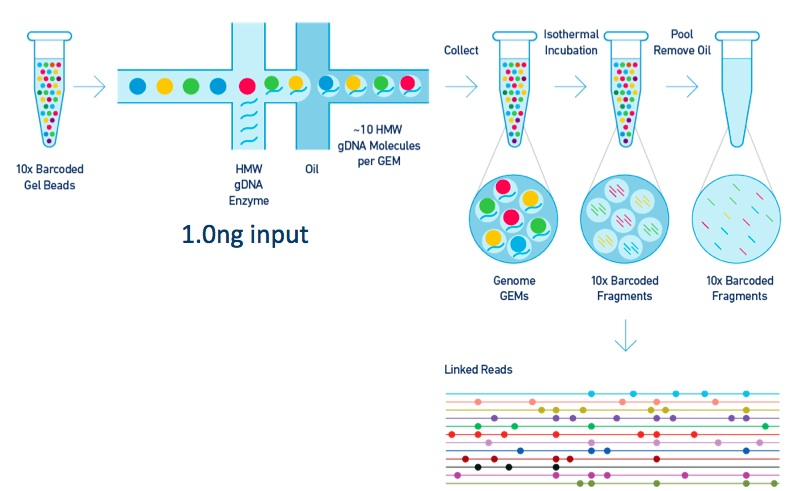
\includegraphics[width=0.65\textwidth]{linkedreads.jpeg} \label{fig:a}
} \\
\sidesubfloat[]{
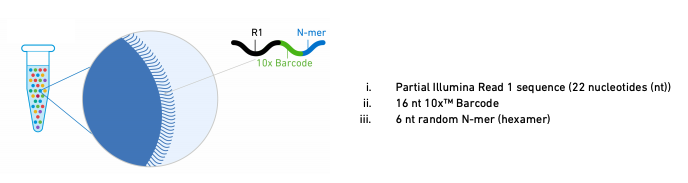
\includegraphics[width=0.65\textwidth]{gem.png} \label{fig:b}
} \\
\sidesubfloat[]{
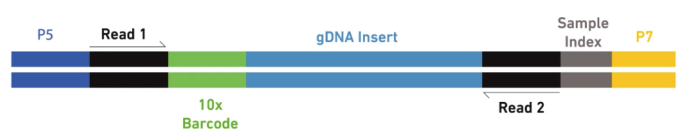
\includegraphics[width=0.65\textwidth]{construct.png} \label{fig:c}
}
\floatfoot{\small{\textbf{a)} outlines the microfluidic system to create the Gel bead in reverse emulsion. \textbf{b)} shows the gel bead oligo setup and \textbf{c)} diagrams the final construct. (image credits to 10xgenomics website)}}
\end{centering}
\end{figure}

\par{
While 10x Genomics Linked reads are used in Chapter 4 for phasing and phased assembly, the technology is no longer offered by that company. More recently, bead based systems have been developed that do not require a microfluidic system. In solution with microbeads, long DNA molecules tend to wrap around a single bead\cite{beadphasing}\cite{LFR}. Separately, Tn5 transposase has been used to insert adapter and barcode sequences at high frequency into genomic DNA\cite{cptseq}. With these ideas combined, Frank Chan's group has developed a technique called Haplotagging which uses microbeads bound to Tn5 transposase with one of 85 million molecular barcodes and Illumina sequencing adapters creating linked read libraries for a fraction of the price in a single tube\cite{haplotagging}.
}

\subsection{Third generation sequencing: long reads}\label{section:longreads}

\subsubsection{PacBio}

\par{
Pacific Biosciences (PacBio) uses microscopic wells known as zero-mode waveguides (ZMWs) along with single molecules of DNA and DNA polymerase to optically measure fluorescent nucleotides as they are incorporated by the polymerase. This is known as single molecule real-time sequencing (SMRT sequencing). The DNA template is prepared with hairpin adapter sequences known as the SMRTbell adapters. This allows for multiple passes of the same DNA molecule. Initially, polymerase nucleotide incorporation and optical measurement speed were limited. That combined with the rate at which molecules dissociate from the ZMW limited the number of times long molecules could be sequenced to once or just a few times. This results in long, but noisy reads with roughly 15\% error rate\cite{pacbio}\cite{blasr}\cite{clrerror} known as continuous long reads (CLR). The PacBio data used in Chapter 3 is CLR data. More recently, advances in the speed of polymerase nucleotide incorporation and optical measurements have allowed for many passes of the same long molecules. This allows for circular consensus sequencing (CCS aka HIgh FIdelity sequencing or HIFI) across these multiple passes and much higher accuracy (<<1\% error rate on average) while maintaining true single molecule sequencing\cite{HIFI}. Over the past few years, PacBio data---both CLR and CCS---has revolutionized genome assembly and is now used routinely for generating high quality reference genome assemblies\footnote{While I would take no credit for HiFi technology, it is poorly known the contribution that my good friend Brendan Galvin had on it. I don't know the full history, but when Brendan was working for PacBio in late 2017, he called me and offered three options for possible improvements to long read sequencing. Among these was longer read CCS data---he estimated the possibility of 10kb CCS reads. He asked me among his three options, which one would have the biggest impact on genome assembly. I responded that 10kb accurate reads would revolutionize the world of assembly. Within a year and a half of that conversation, this became a reality. Of course this was not entirely Brendan's doing either, but between his technical contributions and internal advocation for the technology, I am convinced he played a large role. This is just one of several major contributions to the field he has had.}. In chapter 4, I use PacBio HiFi data for phased assembly.
}

\begin{figure}[htbp!]
\caption{Circular consensus sequencing}
\label{figure:ccs}
\begin{centering}
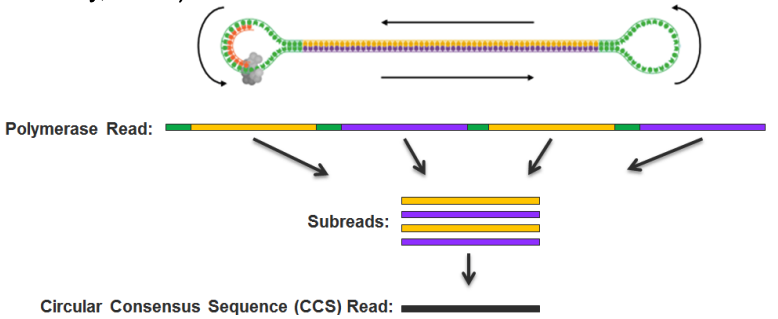
\includegraphics[width=0.65\textwidth]{CCS.png}
\floatfoot{\small{Diagram outlining circular consensus sequencing (credit: PacBio website).}}
\end{centering}
\end{figure}

\subsubsection{Nanopore sequencing}

\par{
The idea of reading single molecules of DNA by the current changes as a molecule translocations through a protein nanopore in a bilipid membrane by electrophoresis goes back to the 1980s\cite{nanopore1} but took twenty-five years of work before Oxford Nanopore brought the technology to market\cite{nanopore2}\cite{nanopore3}. Because more than one base is inside the nanopore at each timepoint and the past current fluctuations affect the current signal, complex models must be used to interpret this data\cite{nanocall}\cite{deepnano}. With these models and improvements in the protein nanopore, sequence accuracy has been reported as high as 92\%, but is sequence context dependent. Read lengths for this technology are limited to the input DNA size and reads have been reported as long as 2.3Mb\cite{longlong}\cite{ultralong2}. This data is not used in this thesis, but is an important aspect of the third generation of DNA sequencing and has been used successfully in the telomere to telomere project\cite{T2T2}.
}

\subsection{Reference Genomes}

\par{
Despite their limitations, reference genomes enable a host of downstream analyses. They provide a common coordinate system by which to say certain genetic variants in one genome are the ``same'' or different from one another. This allows one to compare multiple genomes and associate certain genetic variants with phenotypes.
}

\subsubsection{Resequencing}

\par{
Reference genomes also allow much more inference to be made from the cheap and high throughput next-gen sequencing technology. Instead of generating the entire sequence of each new individual \textit{de novo}, one can create short or long reads and map them onto a reference genome with the assumption that the reference is similar enough to the genome of interest that the mapping is globally correct. Aligning a small sequence with a very large sequence would be computationally expensive with traditional alignment algorithms\cite{smithwaterman}\cite{needlemanwunsch}. Many algorithms and data structures have focused on the ability to quickly find all locations in one large reference or database or sequences a new query sequence will match well such as the suffix tree and suffix array, fm-index, burrows wheeler index, and minimizers. A full review of these is out of the scope of this thesis\cite{suffixarray}\cite{suffixtree}\cite{fmindex}\cite{fmindex2}\cite{bwa}\cite{blat}. One of the more recent of these is relevant to this thesis which is the minimizer. In a sliding window of sequence of size $W$, the minimum (lexicographically or by hash value) sequence of length $K$ is stored for each window\cite{minimizers}. Because adjacent windows often have the same minimum kmer, these can be stored efficiently. And it guarantees a representative kmer at least every $W$-$K$ bases. These have been used in genome assembly, read mapping, among others\cite{LSH}\cite{minimap2}\cite{mashmap}. In a somewhat related idea, if one wants a subset of kmers and does not require the locality guarantee, one can take the kmer hash or two-bit encoding value modulo some number and use only kmers where the resulting value meets some criteria (eg. kmer-hash \% 2 == 0 retains half of the kmers)\cite{modimizer}. These are used in chapter 4 in phased assembly and scaffolding to sparsely sample homozygous kmers to cover areas of the genome with large homozygous stretches. 
} 

\par{
Once one has determined the location to map a read to in the genome, a full smith waterman of the sequence to that region of the genome is done\cite{smithwaterman}. One can then inspect the differences between the genome of interest and the reference genome to call genetic variants. When one parental chromosome contains one allele and the other parental chromosome contains a different allele, this site is said to be heterozygous and results in roughly half of the reads that are sampled contain each allele.\cite{freebayes}\cite{gatk}.
}

\subsection{Haplotype phasing}\label{section:phasing}

\par{
The genetic variants for these individual(s) are generally called in a localized fashion. Some haplotype information may be used, but due to the read lengths of next-gen sequencing, they usually are fairly isolated from one another. Determining which alleles occur on the same chromosome and which occur on the alternate parental chromosome was historically termed haplotype assembly but today is called haplotype phasing. Methods for haplotype phasing generally fall into two categories---population level haplotype estimation and individual genome haplotype phasing. 
}

\subsubsection{Statistical}

\par{
Because chromosomal recombination is relatively rare, alleles close to one another in the genome will generally cooccur across individuals in the population. Given the genotypes of many individuals, it is possible to statistically determine the most likely set of haplotypes in the population\cite{shapeit4} and use this for genotype inference of other variants not sampled in a sparsely sequenced dataset.
}

\subsubsection{Direct / Read based}

\par{
Haplotype phasing across large regions of the genome requires long range genetic information not present in next-gen sequencing. If one considers the graph where heterozygous variants are nodes and reads containing two heterozygous variants create an edge between those nodes, it is only possible to phase variants with respect to one another in connected components in that graph. With contiguous reads such as those generated by PacBio or ONT, the potential sizes of regions that can be phased are limited by the length of homozygous regions. Evolution can naturally create large regions of homozygosity through harsh selective pressures sweeping the haplotype landscape in particular regions\cite{homozygosity}. This limits the ability of contiguous or localized technologies to generate chromosome scale haplotype phasing. By this reasoning, longer reads generate longer phase-blocks, linked reads generate longer phase blocks due to their longer molecule length, and chromosome scale data such as Hi-C has the ability to infer chromosome scale haplotypes\cite{falconphase}. Many algorithms have been developed for haplotype phasing for different data types or combinations of data types and employ search methods, dynamic programming optimization, graph theoretical approaches, and more. These include HapCut2\cite{hapcut2}, Whatshap\cite{whatshap}, Longranger\cite{10xlinked}, and many more. In chapter 4 I use haplotype phasing and the phasing consistency of molecules across multiple heterozygous variants as evidence that those variant loci are physically linked in both haplotypes in the genome.
} 
\par{
One can also phase individuals based on pedigree information. With the genotypes from the mother, father, and child (or larger pedigree datasets), one can phase variants in the child in all cases except when all three are heterozygous\cite{phasingreview}. One can also combine read based phasing with pedigree information\cite{Garg2016}.
}

\subsection{Creating reference genomes}

\par{
Physical and technical limitations make reading whole chromosomes a practical impossibility. Therefore, to recover the sequence of the genome often requires sampling reads from the genome randomly until one has with high probability covered the genome more than once in almost all regions\cite{LanderWaterman} in a method known as `shotgun' sequencing. Using the sequence similarity of multiple reads, one can build a consensus sequence of the underlying genome. This process is known as `assembly'.
} 

\subsubsection{The old way}

\par{
Before next-gen or third generation sequencing was available, there were several massive efforts to sequence genomes, but they were limited to human, important crops, and model organisms due to their cost and time\cite{genomeproject}\cite{mousegenome}\cite{maizegenome}. In these projects, BACs and other vectors were used to clonally amplify large sections of the genome. Shorter sequences from these would then be subcloned and Sanger sequencing was used to produce reads from each end of these, and each BAC would be assembled separately. At the end, all BAC sequences would be assembled together, often with the aid of a physical map. While costly, this method had several benefits over the whole genome shotgun method used in the privately funded human genome effort and over the later next-gen shotgun assemblies. The ability to deal with 150-200kb at a time means that many repeats that would make the assembly process difficult are absent as they may occur in a separate BAC clone. The clonal nature of this strategy also means that only one haplotype is being sampled in a given BAC and the heterozygosity that may make assembly difficult is also not present. And the Sanger sequencing read lengths also spanned small repeat structures that the later next-gen sequencing did not. These projects, while costly, produced high quality reference genomes for the most important organisms to the human species and are still being used today.
}

\subsubsection{The dark times}

\par{
In the age of next-gen sequencing, genome assembly was initially still popular. The low cost of sequencing promised personal genomes and the ability for every lab to sequence and assemble the genome of their organism of interest. Despite a massive amount of research going into assembly algorithms, \textit{de novo} genomes produced with this technology were never even close to as high quality as the ones produced by the BAC+Sanger sequencing methods of the previous generation\cite{illuminashit}\cite{gage}. Over time, interest in genome assembly waned both from the perspective of assembly algorithm development as well from people wanting to assemble new genomes as the results were so fragmented and error prone as to be of little downstream use\cite{assemblethon}.
}

\subsubsection{A new hope}

\par{
Long single molecule read technologies have been around and commercialized since the 2010, but due to cost, scaling, and the computational difficulties of dealing with high error reads took some time for widespread adoption for genome assembly\cite{HGAP}. But as cost came down, throughput scaled up, and tools for assembling this data improved\cite{falcon}\cite{redbean}\cite{canu}, this technology rapidly became the goto for \textit{de novo} genome assembly. Initially this was usually paired with a next-gen short read dataset used to polish the assembly and/or reads prior to assembly, but eventually partial order alignment multiple sequence alignment\cite{partialorder} was used for polishing by the noisy long reads themselves\cite{quiver}. More recently, PacBio's improvements to the nucleotide incorporation speed of the polymerase along with their circular consensus technology has allowed for many passes of a long single molecule which can then self polish with these same algorithms. This produces high accuracy long reads which have even further revolutionized genome assembly\cite{hifi}. This, combined with Hi-C scaffolding now routinely produces reference quality genomes in full chromosome scaffolds. However, some problems still exist for certain genomes. Until recently, long read technologies required more DNA input than could be extracted from single small organisms. But due to recent advances in library preparation, DNA requirements have come down substantially and in Chapter 3 I describe the first high quality assembly of a single mosquito. Also, many organisms are highly heterozygous and this creates difficulties in the assembly process. In Chapter 4, I describe methods for turning the problem of heterozygosity into an advantage by using phasing consistency between multiple heterozygous sites as a signal for physical linkage in phased assembly and phased scaffolding.
}

\subsection{Assembly algorithms}

\par{
Outside of some enzymatic reaction modeling I did in high school, the problem of genome assembly was the first problem in computational biology that I was introduced to and arguably one of the most important problems to the field. While the problem naturally lends itself to the pure computer scientists and mathematicians, the peculiarities of how genomes evolve tend to defy most basic assumptions. Not only is genomic sequence not random, but many structures seem designed to make the problem harder. Transposable elements and large segmental duplications, viral insertions and trinucleotide expansions, low GC content and homopolymers, centromeric repeats and telomeric repeats are just a few of the challenges the genome poses to the problem of assembly. At its most basic, the problem is simple. Find similar overlapping sequences. Infer that those sequences most likely originated from the same locus in the genome. Create a larger contiguous sequence representing the underlying genome and repeat. The problems arise when this inference is false. These algorithms have evolved over time and with the data types available, cheapest, or most promising at the time.
}
\subsubsection{Overlap, Layout, Consensus}

\par{
The first assembly algorithms were known as ``overlap, layout, consensus'' algorithms due to their three primary steps. They first do an all vs all alignment of the reads. While this seems computationally costly, due to exact match hashing of smaller subsequences as a filter, only reads very likely to arise from the same genome locus well will be aligned\cite{OLC}. These overlaps can then be used to create an ordering, or layout, of these reads. This layout was then used to generate a consensus either through multiple sequence alignment or heuristics\cite{gene1}. This method was used for many years including on large sequencing efforts such as the Human Genome Project\cite{genomeproject}. Implementations of this strategy include PHRAP\cite{phrap}, TIGR\cite{tigr}, GigAssembler\cite{gigassembler} (used in the human genome project), and the Celera assembler\cite{Myers2000}. The Celera assembler was developed for and used in the privately funded human genome project\cite{privategenome} and many other genome projects of this era. In the modern era, Falcon and Canu are overlap, layout, consensus algorithms build for long noisy reads\cite{falcon}\cite{canu} and HiCanu for long accurate reads\cite{HICANU} and have generated many high quality genome assemblies\cite{singlemosquito}.
}

\subsubsection{de Bruijn graphs}
\par{
One of the earliest formalizations of assembly as a graph theoretical problem was in the late 1980s in the context of sequencing by hybridization (SBH)\cite{SBH}. In sequencing by hybridization, one would expose many copies of single stranded DNA of interest to an array of microwells with different oligonucleotides. The unbound DNA would then be washed away and a reporter system was used to determine which wells the DNA bound to. This indirectly created the later microarray SNP-chip technology. While this technology never proved feasibly scalable for both laboratory and information theoretical reasons\cite{Preparata}\footnote{From 2011-2013 I worked at Nabsys, a company that was attempting initially to create a positional sequencing by hybridization\cite{positionalSBH} technology where DNA would be tagged with oligos and translocated by electrophoresis through a nanopore and the oligo locations would be read. If this was done for all of the oligos of a certain length, the positional information would potentially solve the information content problem for longer sequences. This failed horribly due to several limitations. The company continued on to create a digital ordered restriction map technology\cite{nabsyspatent} creating similar data to that produced by bionanogenomics but less successful. While the technology was ultimately a failure, my time there was an incredible learning experience.}, it did motivate Pavel Pevzner to pose assembly as an Eulerian path on a de Bruijn graph of the sequences. In SBH, the oligos used were short due to the maximum number of microwells possible and the total number of possible oligos of a given length ($4^{k}$ where k is the length of the oligo). A graph was constructed such that kmers (at the time, these were referred to as I-tuples, but I will use the modern terminology) with overlapping k-1 sequences would have edges between them. A Eularian path on this graph represents a linear assembly of the sequence. Later, with next-gen short reads, this idea was given new life with Pevzner and Waterman\cite{Pevzner2001} creating an assembly algorithm Euler based on this idea. With reads as opposed to short oligo microarray hits, one uses all subsequences of length $k$ and constructs the same type of graph as with SBH\cite{Zerbino2008}\cite{abyss}\cite{iqbal}. The obvious downside of these techniques is the loss of information by breaking the read into shorter sequences. However, this can be mitigated by reconsidering the reads and read pair information to further resolve the graph\cite{allpaths}\cite{discovar}. These methods are only applicable to data types with relatively high accuracy reads as the length of a kmer of any length in PacBio CLR or ONT reads would not be a true kmer with high probability. Although Jue Ruan and Heng Li used a fuzzy de Bruijn graph approach for noisy long reads.
}

\subsubsection{String graphs}

\par{
The string graph is a data structure representing the idealized assembly graph and was described by Gene Myers in 2005\cite{Myers2005}. It uses the full read lengths and overlaps between reads are collapsed into a single sequence. Thus, if there are repeats longer than the read length, these will be collapsed and unique sequence will create loops between repeats. Jared Simpson and Richard Durbin created a compressed version of this dataset and an assembly algorithm based on it using the FM-index\cite{fmindex2}\cite{fmindex}\cite{SGA}. This allowed for the use of the full length of the reads without complex and costly read pair threading algorithms on the de Bruijn graph and the compression reduced the memory requirements to the point that mammalian genomes could be assembled on commodity hardware of the time. HifiAsm represents a phased string graph built on PacBio Hifi accurate long read data\cite{hifiasm} and produces some of the highest quality assemblies today.
}


\subsubsection{Repeats, Heterozygosity, and Errors}

\par{
While tremendous progress has been made in genome assembly through improvements in both the data and algorithms, problems still exist. In the process of creating overlaps, one will encounter inexact homology due to either inexact repeats, heterozygosity, or sequencing errors. In the graph methods that only collapse exact matching sequence, these inexact homologous sequences arising from these create complex graph structures that either need to be resolved or the final sequence assembly will be fragmented\cite{assemblyissues}. Many organisms are much more heterozygous than humans, who went through a population bottleneck in recent evolutionary history\cite{bottleneck}. While much of the exact repeat problem has been solved due to long accurate reads spanning such repeats, inexact but highly homologous repeats exist on the scale of megabases\cite{segmentaldups}. In haploid assembly, any inexact homology is either due to errors or repeats. In diploid and polyploid assembly, inexact homology can come from paralogous sequences, heterozygosity, or sequencing errors. Incorrectly inferring one as another can create misassemblies or retained haplotypes assembled separately which are generally intended to be collapsed in a reference genome for the downstream application of resequencing. Several methods have been created to combat these problems.
}
\subsubsection{Trio assembly and trio binning}
\par{
One way to reduce the problem of heterozygosity versus repeats is to add haplotype phasing information to the process. In section \ref{section:phasing}, I discussed haplotype phasing via pedigree genotypes. With this information, one can more easily distinguish between heterozygosity and paralogous sequences. In the age of next-gen sequencing, Malinsky, Simpson, and Durbin, created Trio-SGA, an algorithm utilizing parental and child information in the string graph based algorithm to deliver higher quality assemblies\cite{trio-sga}. More recently, with the reduced costs of long read sequencing technologies, instead of embedding the knowledge of the pedigree information into an assembly algorithm, trio-binning\cite{triobinning} separates the long reads by haplotype prior to haploid assembly of each haplotype. Because long reads generally span multiple heterozygous variant cites, trio-binning uses the kmer difference between the paternal dataset and maternal dataset to categorize reads as maternal, paternal, or uncategorized. Each bin of haplotype reads, along with the uncategorized reads, are then assembled independently producing highly contiguous and accurate genome assemblies. However, this requires pedigree data which is not feasible for many species in a large project such as the Darwin tree of life and the Earth biogenome project.
}

\subsubsection{Haploid assembly: Hytaditiform moles, seeds}

\par{
In cases where it is possible to assemble haploid data, it is clearly advantageous. The telomere to telomere (T2T) consortium has used multiple technologies to sequence a human cell line derived from the haploid CHM13 hytaditiform mole\cite{T2T2}. While this does not represent a viable human genome, it is likely the most complete and accurate sequence of a human genome to date. In some other areas, tissues are clonally haploid with enough material to create a sequencing library. In many conifer species, the seeds within pine cones are haploid and can be used as source material for genome assembly where other material may be polyploid\cite{coniferhaploid}.
}
\subsubsection{Phased assembly}

\par{
Another option for combatting the heterozygosity vs paralogous sequence problem is building haplotype phasing into the assembly algorithm and explicitly assembling both haplotypes. Many algorithms have attempted this in the past including Falcon\cite{falcon} and trio-sga\cite{trio-sga}, but until recent data improvements, this has proven difficult. One approach used in DipAsm, was to create an initial assembly, haplotype phase that assembly, and then use that phasing to split haplotypes prior to haploid assembly---a process akin to trio-binning but without the pedigree information\cite{dipasm}. Another method is to create a de Bruijn graph or string graph via short reads and align long reads onto that graph to both phase the graph and assemble both haplotypes\cite{Garg2018}. And yet another approach employed in HiFiAsm is to create a phased string graph directly from the long accurate HiFi reads\cite{hifiasm}. In chapter 4, I present a method using haplotype phasing consistency to create phased assemblies and phased scaffolds.
}

\subsection{Post assembly manipulations}
\subsubsection{Polishing}
\par{
Especially when assembling with long noisy reads, and sometimes with other technologies, a post assembly step of polishing can improve base quality. With long noisy reads such as PacBio CLR or ONT, one can polish with the reads themselves\cite{arrow}\cite{nanopolish} or one can use a short read dataset to polish the final assembly\cite{pilon}.
}
\subsubsection{Haplotig purging}

\par{
Because one of the primary downstream applications of reference genomes is resequencing, and it is undesirable for the two haplotypes to compete for read mapping, we generally want to produce an assembly with only one haplotype. If the haplotypes are different enough, assemblers may assemble portions of haplotypes as separate contigs rather than collapsing them. Several tools have been made to remove these ``haplotigs'' or ``haplotypic'' sequence using both sequence similarity as well as coverage of reads mapped to the pre-purged contigs\cite{haplomerger}\cite{purge}\cite{purgedups}.
}
\subsubsection{Scaffolding}

\par{
In most cases, contigs resulting from the assembly process are not chromosome length, and if further information is available, we would like to order and orient them with or without gaps in their chromosomal context. Paired end reads, long reads, linked reads, Optical maps, and HiC have been used for this purpose over the years\cite{scaffoldingreview}\cite{scaff10x}\cite{SALSA}. The longer range the data is, generally the better it is for scaffolding to span whatever gaps may exist between contigs. So in the modern era, HiC is the preferred data type for scaffolding. In chapter 4, I present a method for phasing and phasing aware assembly scaffolding.
}
\subsubsection{Gap filling}

\par{
Gaps may exist either due to contigs being scaffolded together with a gap between them or through the assembly process itself. These can sometimes be filled by aligning reads across the ends of each contig on either side and creating a consensus sequence for the gap\cite{pbjelly}. More recently, ultralong ONT reads have been used to fill gaps in projects like the T2T project\cite{ultralong1}\cite{ultralong2}.
}

\subsection{Assembly validation and curation}

\par{
While the modern assembly process is much more automated than it used to be, some validation and curation is still necessary for the highest quality genomes. Today, curators use semi-automated tools to assess haplotig retention, contamination, find and bread misassemblies and order and orientation errors in scaffolding\cite{curation2}. Assembly completeness and haplotig retention is assessed by orothology of genes to known sets of genes using Benchmarking Universal Single-Copy Orthologs (BUSCO)\cite{BUSCO}. Kmer methods such as KAT plots\cite{KAT} can be used to assess heterozygosity, error rate, and haplotig retention. HiC data is visualized on a heatmap and used to correct scaffolding errors, create new scaffolding joins, and find potential misassemblies\cite{juicer}\cite{higlass}\cite{juicebox}. Coverage of reads aligned to the assembly along with G/C content and database searches of sequences are used to find contamination of other organisms in your sample and assembly\cite{blobtools}\cite{blobtoolkit}.
}

\par{
In the following chapters I will present several methods for using genetic variation to demultiplex single cell RNAseq mixtures and improve genome assembly and scaffolding. I will attempt to use the word ``I'' when I have done the work alone and ``we'' when it was done in collaboration with others.
}

